\section{Self-Suspending Tasks in Multiprocessor Synchronizations}
\label{sec:syn}

In this section, we consider multiprocessors subject to \emph{partitioned fixed-priority (\pfp)} scheduling, and review the general analysis strategies for tasks that synchronize access to shared resources (\eg, shared I/O devices, communication buffers, or scheduler locks) with suspension-based locks (\eg, binary semaphores). Unfortunately, some of the misconceptions surrounding the analysis of self-suspensions on uniprocessors also spread to the analysis of partitioned multiprocessor real-time locking protocols. In particular, as we show with a counterexample, the analysis framework to account for the additional interference due to \emph{remote blocking} first introduced in \cite{lakshmanan-2009}, and reused in several other works~\cite{zeng-2011,bbb-2013,yang-2013,kim-2014,han-2014,carminati-2014,yang-2014},  is flawed. Finally, we present a straightforward solution for these problems. 

\subsection{Existing analysis strategies}
\label{sec:papers}

\pfp scheduling is a widespread choice in practice due to the wide support in industrial standards like POSIX\todo{To my understanding, POSIX mandates fixed-priority scheduling, but is silent on global \vs partitioned scheduling.} and AUTOSAR, and in many RTOSs like VxWorks, RTEMS, ThreadX, \etc Under \pfp scheduling, each task has a fixed base priority and is statically assigned to a specific processor, and the tasks on each processors are scheduled as in uniprocessors. At runtime, a resource-holding job may be assigned a temporarily elevated effective priority according to the employed locking protocol. Thus on each processor, the ready job with highest effective priority is scheduled.\todo{Why are effective priorities relevant here? Just cut it?} 

Under partitioned scheduling, a resource accessed by tasks from different processors is called a \emph{global resource}, otherwise it is called a \emph{local resource}. When a job requests a global resource, it may incur \emph{remote blocking} (\ie, it may self-suspend) if the global resource is held by a job on another processor. Also, a job may incur \emph{local blocking} if it is prevented from being scheduled by a resource-holding job of a lower-priority task on the same processor.\todo{This is confusing to read: when a job incurs local blocking, does it not suspend itself? What is the difference between a self-suspension and local blocking (which also involves suspending)? This needs clearer terminology.} From the perspective of local schedule on each processor, remote blocking, caused by external events (\ie, depends on the schedule on the other processors), pushes the execution of higher-priority tasks to a later time point, thus can cause additional interference on lower-priority tasks. 

A safe yet pessimistic strategy is to convert remote blocking into computation. Accordingly, the remote blocking incurred by each higher-priority task is counted as part of interference. \citet{block-2007} first used this strategy for partitioned \emph{earliest deadline first (EDF)} scheduling;  \citet{lakshmanan-2009} also adopted this approach in their analysis of ``virtual spinning,'' where\ldots\todo{give the reader a hint what this means} An alternative is to bound the effects of deferred execution due to remote blocking. In the original utilization-based analysis\todo{What is a ``utilization-based analysis''? This is not a well-defined concept.} for multiprocessor locking protocols~\cite{rajkumar-1990,RSL:88}, the additional interference from a task $\tau_i$ on task $\tau_k$ was counted as part of blocking for $\tau_k$, and was bounded by the maximum remote blocking or the WCET of $\tau_i$ (whichever is smaller).\todo{This is confusing and unclear. Please clarify. Perhaps just show the analysis? Or omit its discussion? What is the relevance to the point of this paper? It's not flawed, so why even bring it up?} Recently, \citet{lakshmanan-2009} proposed the following response-time analysis framework that takes into account the amount of remote blocking to bound the worst case interference.\todo{Is this exactly the formula from \cite{lakshmanan-2009}? }

\begin{align}
\label{eq:wcrt}
R_k^{n+1} = C_k + B_k^r + B_k^l + \sum_{\tau_i \in \fun{hp(k)} \cap P(\tau_k)} \left \lceil \frac{R_k^n + B_i^r}{T_i} \right \rceil \cdot C_i.  
\end{align}
where $R_k^0 = C_k + B_k^r$, and $\tau_k$ is schedulable if $R_k^{n+1} = R_k^n < D_k$. 

In \equref{wcrt}, $B_k^r$ (respectively, $B_k^l$) is an upper bound on the maximum remote (respectively, local) blocking that a job of $\tau_k$ incurs, $\fun{hp(k)}$ denotes the tasks with higher priority than $\tau_k$, and $P(\tau_k)$ denotes the tasks that are assigned on the same processor as $\tau_k$. The additional interference on $\tau_k$ due to the remote blocking incurred by each higher-priority task is captured in the analysis according to the fourth term in \equref{wcrt}.

Under this analysis framework, $\left \lceil \frac{R_k + B_i^r}{T_i} \right \rceil \cdot C_i$ is used as an upper bound on the total interference of $\tau_i$ on $\tau_k$. This analysis approach was reused in \cite{yang-2013,kim-2014,carminati-2014,yang-2014} to analyze (several variants of) the \emph{multiprocessor priority ceiling protocol (\mpcp)}. The response-time analysis framework (\ie, \equref{wcrt}) was also reused in \cite{zeng-2011,bbb-2013,han-2014} to compare the schedulability performances between different locking protocols under \pfp scheduling. 

Unfortunately, the analysis approach based on \equref{wcrt} fails to guarantee a safe response time bound in certain corner cases, as can be demonstrated with the following counterexample.

\subsection{A counterexample}

We show the existence of a schedule in which a task that is considered schedulable according to the analysis in \cite{lakshmanan-2009} is in fact unschedulable.

\begin{figure}[!ht]
\captionsetup{belowskip=-1pt}
\begin{center}
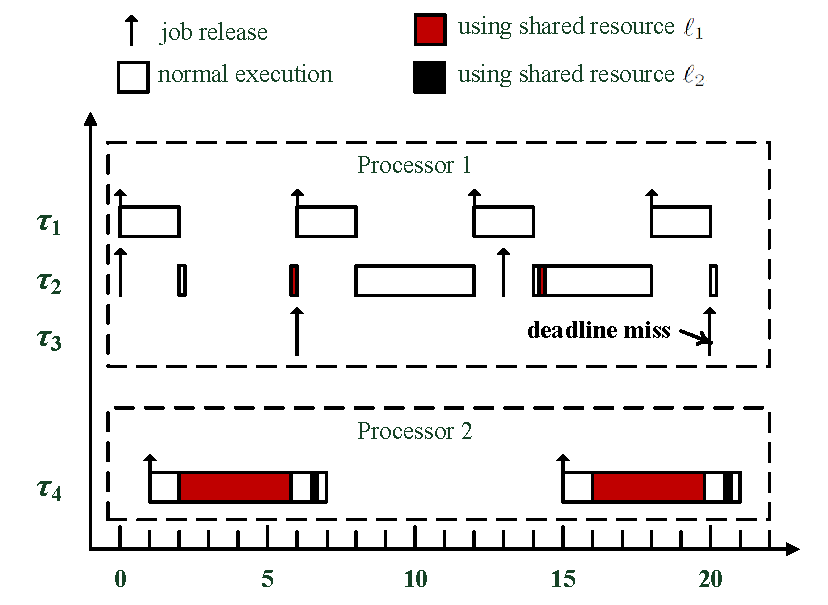
\includegraphics[width=12cm]{Counterexample}
\caption{An example schedule in which the first job of $\tau_3$ misses its deadline. 
\iffalse
The first job of $T_2$, denoted by $J_{2,1}$, releases at time $t=0$ and is scheduled at time $t=2$ when the first job of $T_1$ finishes.
At time $t=2+\varepsilon$, $J_{2,1}$ requests a shared resource $\res_1$ and incurs remote blocking (self-suspension) because $\res_1$ has been locked by $T_4$ at time $t=2$.
$J_{2,1}$ gets access to $\res_1$ until time $t=6-\varepsilon$. 
At time $t=6$, $J_{2,1}$ release $\res_1$ and is preempted by the second job of $T_1$, meanwhile, a job of $T_3$ releases. 
$J_{2,1}$ finishes at time $t=12$, and the second job of $T_2$, denoted by $J_{2,2}$, releases at time $t=13$. 
$J_{2,2}$ is scheduled at time $t=8$. 
It gets access to $\res_1$ at time $t=14+\varepsilon$ without incurring remote blocking (self-suspension), and it is always executing during $t \in [14,18)$.
Then, the forth job of $T_1$ releases, and it is executing during $t \in [20,22)$.
At time $t=22$, $J_{2,2}$ resumes, and the job of $T_3$ misses its deadline.
\fi
}
\label{fig:counterexample}
\end{center}
\end{figure}

\begin{table} 
\centering
\caption{Task parameters}
\begin{tabular}{|c|c|c|c|c|c|c|} \hline
$\tau_k$ & $C_k$ & $T_k$ ($= D_k$) & $N_{k,1}$ & $L_{k,1}$ & $N_{k,2}$ & $L_{k,2}$\\ \hline
$\tau_1$ & 2           & 6  & 0 & 0 & 0 & 0\\ \hline
$\tau_2$ & $4+2\epsilon$ & 13 & 1 & $\epsilon$ & 0 & 0\\ \hline
$\tau_3$ & $\epsilon$    & 14 & 0 & 0 & 1 & $\epsilon$\\ \hline
$\tau_4$ & 6             & 14 & 1 & $4-\epsilon$ & 1 & $\epsilon$\\ \hline
\end{tabular}
\label{tab:parameters}
\end{table}

%\multicolumn{2}{c}{} 
%\multirow{2}{*}{Progress Mechanism}


Consider four implicit deadline sporadic tasks ${\tau_1, \tau_2, \tau_3, \tau_4}$ (with parameters listed in \tabref{parameters}),\todo{Is this notation already defined? Do the earlier sections even talk about $N_{k,1}$ and $L_{k,1}$?} ordered by decreasing order of priority, that are scheduled on two processors using \pfp scheduling. $\tau_1$, $\tau_2$ and $\tau_3$ are assigned to processor 1, while $T_4$ is assigned to processor 2. Jobs of $\tau_2$ and $\tau_4$   each once access a shared resource $\res_1$  ($N_{2,1} = 1$ and $N_{4,1} = 1$). Each job of $\tau_2$ uses $\res_1$ for a duration of at most $L_{2,1} = \varepsilon < 1$ time units (an arbitrarily small quantity), and each job of $\tau_4$ uses $\res_1$ for at most $L_{4,1} = 4-\varepsilon$ time units. 

Consider the response-time of $\tau_3$. Since $\tau_3$ is the lowest-priority task on its processor and $\tau_3$ does not request any resource, it does not incur any blocking (\ie, $B_3^l = B_3^l = 0$). With regard to the remote blocking incurred by each higher-priority task, we have $B_1^r = 0$ because $\tau_1$ does not request any global resource. Further, each time when a job of $T_2$ requests $\res_1$, it may be delayed (\ie, self-suspend) for a duration of at most $4-\varepsilon$ before $T_4$ releases $\res_1$. Thus, the maximum remote blocking of $\tau_2$ is bounded by $B_2^r = 4-\varepsilon$ \footnote{In general, =the upper bound on blocking of course depends on the specific locking protocol in use, but in this example, by construction, the stated bound holds under any reasonable locking protocol. Recent surveys of multiprocessor semaphore protocols may be found in \cite{bbb-2013,yang-2015}.}. Therefore, according to \equref{wcrt}, we have\todo{This does not match the definition of the RTA. Please double-check. The term $ R_3^1$ should already contain some ceilings; the iteration starts at $ R_3^0$. }
\begin{align*}
& R_3^1 = \varepsilon + 0 = \varepsilon, \\
& R_3^2 = \varepsilon + 0 + 0 + \left \lceil \frac{\varepsilon + 0}{6} \right \rceil \cdot 2 + \left \lceil \frac{\varepsilon + 4 - \varepsilon}{13} \right \rceil \cdot (4+2\varepsilon) = \varepsilon + 1 \cdot 2 + 1 \cdot (4+2\varepsilon) = 6+3\varepsilon, \\
& R_3^3 = \varepsilon + 0 + 0 + \left \lceil \frac{6+3\varepsilon + 0}{6} \right \rceil \cdot 2 + \left \lceil \frac{6+3\varepsilon + 4-\varepsilon}{13} \right \rceil \cdot (4+2\varepsilon) = \varepsilon + 2 \cdot 2 + 1 \cdot (4+2\varepsilon) = 8+3\varepsilon, \\
& R_3^4 = \varepsilon + 0 + 0 + \left \lceil \frac{8+3\varepsilon + 0}{6} \right \rceil \cdot 2 + \left \lceil \frac{8+3\varepsilon + 4-\varepsilon}{13} \right \rceil \cdot (4+2\varepsilon) = \varepsilon + 2 \cdot 2 + 1 \cdot (4+2\varepsilon) = 8+3\varepsilon.
\end{align*}
 
As a result, $R_3 = 8+3\varepsilon < 14 = D_3$, and $\tau_3$ is considered to be schedulable according to the analysis in \cite{lakshmanan-2009}. However, there exists a schedule, shown in \figref{counterexample}, where $\tau_3$  actually misses a deadline at time~20, which implies that the analysis framework in \cite{lakshmanan-2009} is too optimistic (in certain cases). 

Based on the above discussion, we can infer that the analysis used in \cite{NBN:11}, which ignored the effects of remote blocking on interference and quantified the total interference from a task $\tau_i$ on $\tau_k$ over a duration of length $t$ as $\left \lceil \frac{t}{T_i} \right \rceil \cdot C_i$, was also over optimistic.\todo{This is confusing. It has actually nothing to do with the preceding analysis, but is a different bug altogether. This should be discussed in a little bit more detail, and in its own subsection.} 

\subsection{A Safe Response Time Bound}
\label{sec:safe_bound}

In \equref{wcrt}, the remote blocking of each higher-priority task (\ie, $B_i^r$) is counted in a similar way as release jitter. However, it is not sufficient to count the duration of remote blocking as release jitter (explained in XXX (\emph{this will be explained in previous sectioins})). A straightforward fix is thus to replace $B_i^r$ with a larger value for each higher-priority task (\ie, $\tau_i$) when $B_i^r > 0$.

\begin{lemma}
\label{lem:new_framework}
The worst-case response time of a task $\tau_k$ is upper bounded by the smallest solution of 
\begin{align}
\label{eq:fix}
R_k = C_k + B_k^r + B_k^l + \sum_{\tau_i \in \fun{hp}(k) \cap P(\tau_k) \wedge B_i^r > 0} \left \lceil \frac{R_k + R_i - C_i}{T_i} \right \rceil \cdot C_i
+ \sum_{\tau_j \in \fun{hp}(k) \cap P(\tau_k) \wedge B_j^r = 0} \left \lceil \frac{R_k}{T_j} \right \rceil \cdot C_j.
\end{align}
\end{lemma}

\begin{figure}[!ht]
\captionsetup{belowskip=-1pt}
\begin{center}
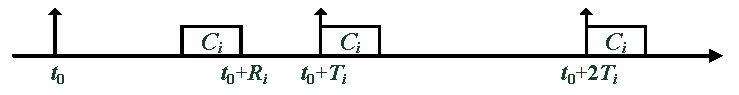
\includegraphics[width=11cm]{max_interference}
\caption{Release pattern for $\tau_i$.}
\label{fig:max_interference}
\end{center}
\end{figure}


\begin{proof}
At any point in time while a job of $\tau_k$ is released but not finishes, it is either \textbf{(i)} executing, \textbf{(ii)} blocked due to tasks on the other processors, \textbf{(iii)} blocked due to tasks on its local processor, or \textbf{(iv)} preempted by higher-priority tasks on its local processor. 
By definition, $C_k$, $B_k^r$, and $B_k^l$ bound the durations of \textbf{(i)}, \textbf{(ii)}, and \textbf{(iii)}, respectively.\todo{I'm following up to here.}

For any higher-priority local task, \ie, $\forall \tau_h \in \fun{hp}(k) \cap P(\tau_k)$, the interference of $\tau_h$ on a job of $\tau_k$ is maximized if the carry-in job executes as late as possible and the following jobs execute as soon as possible, as shown in \figref{max_interference}. Correspondingly, the interference of $\tau_h$ on $\tau_k$ is bounded by\todo{It is not obvious to me that this follows. Please provide a more elaborate, detailed proof. Why is it ok to subtract $-C_h$?} 
\begin{align*}
I_{h,k}^1 = \left \lceil \frac{R_k + R_h - C_h}{T_h} \right \rceil \cdot C_h.
\end{align*}

For any higher-priority local task $\tau_j$ (\ie, $\forall \tau_j \in \fun{hp}(k) \cap P(\tau_k)$) that does not incur remote blocking (\ie, $B_j^r = 0$), $\tau_j$ will not suspend while executing (\ie, does not self-suspend). According to the critical instant theory~\cite{LL-1973}, a job of $\tau_k$ incurs maximum interference by $\tau_j$ when the job releases simultaneously with the release of $\tau_j$.\todo{Why does this theory still apply in the presence of \emph{some} self-suspending tasks? This is not obvious. Please justify in more detail.} Therefore, according to the standard request demand analysis~\cite{audsley-1993}, the maximum interference from $\tau_j$ on $\tau_k$ is given by 
\begin{align*}
I_{j,k}^2 = \left \lceil \frac{R_k}{T_j} \right \rceil \cdot C_j.
\end{align*}

Consequently, the total interference on any job of $\tau_k$ (\ie, the duration of \textbf{(iv)}) is bounded by summing up $I_{i,k}^1$ for each higher-priority local task $\tau_i$ if $B_i^r > 0$, and $I_{j,k}^2$ for each higher-priority local task $\tau_j$ if $B_j^r = 0$, which is given in the fourth and the fifth terms in \equref{fix}.
\end{proof} 

It is noted that, \lemref{new_framework} can also be used to fix the over-optimistic problem in \cite{NBN:11}. Further, since most papers reviewed in \secref{papers} merely reused the over-optimistic analysis framework in \cite{lakshmanan-2009}, an analysis based on \lemref{new_framework} may be used to fix the response-time tests in these papers.